\documentclass[11pt]{article}
\usepackage[margin=0.7in]{geometry}
\usepackage{amsmath,amssymb}
\usepackage{graphicx}
\usepackage{float}
\usepackage{xcolor}
\usepackage{listings}
\setlength{\parindent}{0pt}
\setlength{\parskip}{0.5em}
\lstset{
    language=Python,
    basicstyle=\ttfamily\footnotesize,
    keywordstyle=\color{blue},
    commentstyle=\color{green!50!black},
    stringstyle=\color{red!50!black},
    numbers=left,
    numberstyle=\tiny\color{gray},
    frame=single,
    breaklines=true
}

\begin{document}

\subsection*{1.1(g)}

The problem can be written as a QP
\[
    \min_x \frac{1}{2}x^TQx-b^Tx
    \qquad
    x=\begin{bmatrix}x_1\\x_2\end{bmatrix}
    \qquad
    Q=\begin{bmatrix}1&0\\0&\gamma\end{bmatrix}
    \qquad
    b=\begin{bmatrix}0\\0\end{bmatrix}
\]
Since \(Q\) is positive definite, the optimal solution is
\[
    x^\star=Q^{-1}b=\begin{bmatrix}0\\0\end{bmatrix}
\]

The constant-step plots use \(\eta=0.15\). The level sets satisfy
\[
    x_1^2+\gamma x_2^2=c
\]
For \(\gamma=10\), these are narrow ellipses, so the curvature in the \(x_2\)
direction is much larger than in the \(x_1\) direction. This causes zig-zagging
for both exact line search and constant-step gradient descent.

For constant-step gradient descent,
\[
    x^{(k+1)}=(I-\eta Q)x^(k)
\]
so
\[
    x_{2}^{(k+1)}=(1-\eta\gamma)x_{2}^{(k)}
\]
Zig-zagging begins when \(1-\eta\gamma<0\). Convergence
requires \(|1-\eta\gamma|<1\), which gives \(0<\eta<2/\gamma\). Then, for
\(\gamma=10\), \(\eta=0.15\) zig-zags but still converges, while steps larger
than \(0.2\) diverge. For \(\gamma=1\), the level sets are circular and exact
line search reaches the optimum in one step.

\begin{figure}[H]
    \centering
    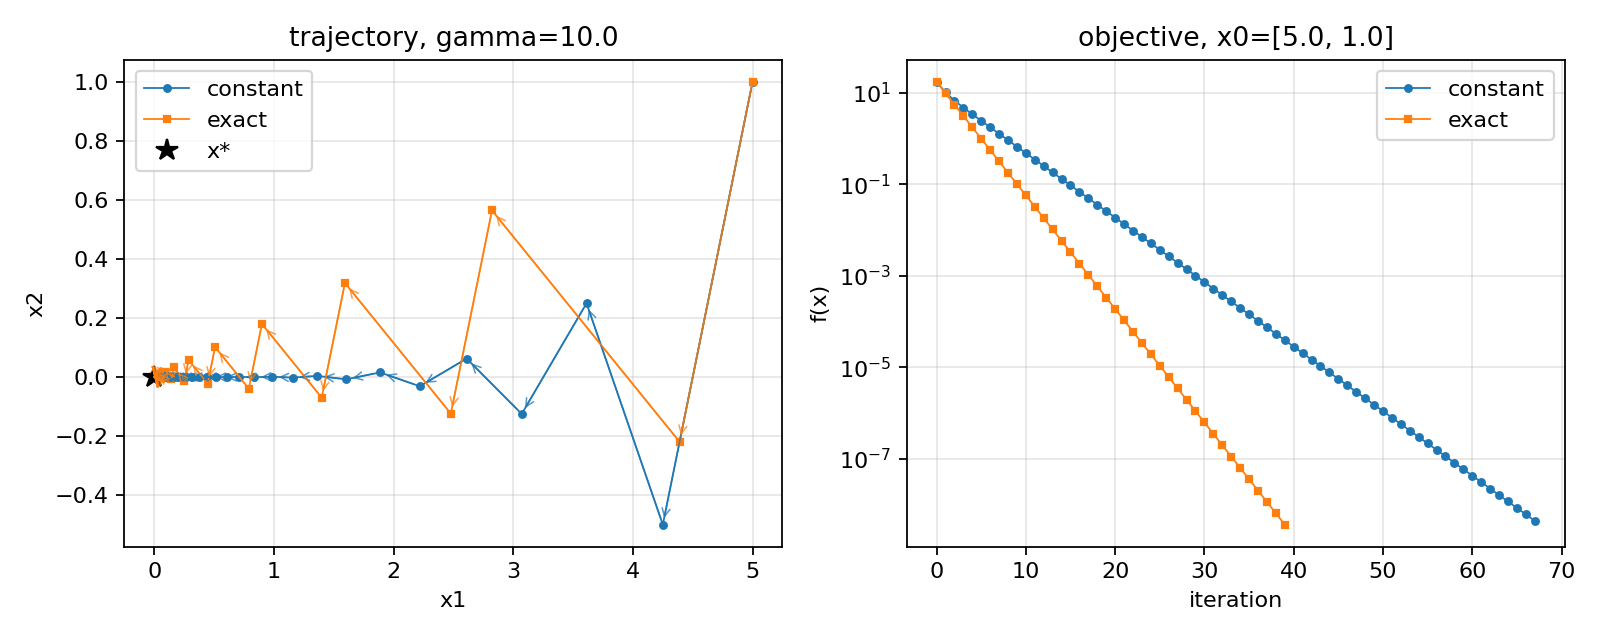
\includegraphics[width=0.82\textwidth]{code/p1_gamma10_x0_5_1.png}
    \caption{\(\gamma=10\), \(x^{(0)}=(5,1)\).}
\end{figure}

\begin{figure}[H]
    \centering
    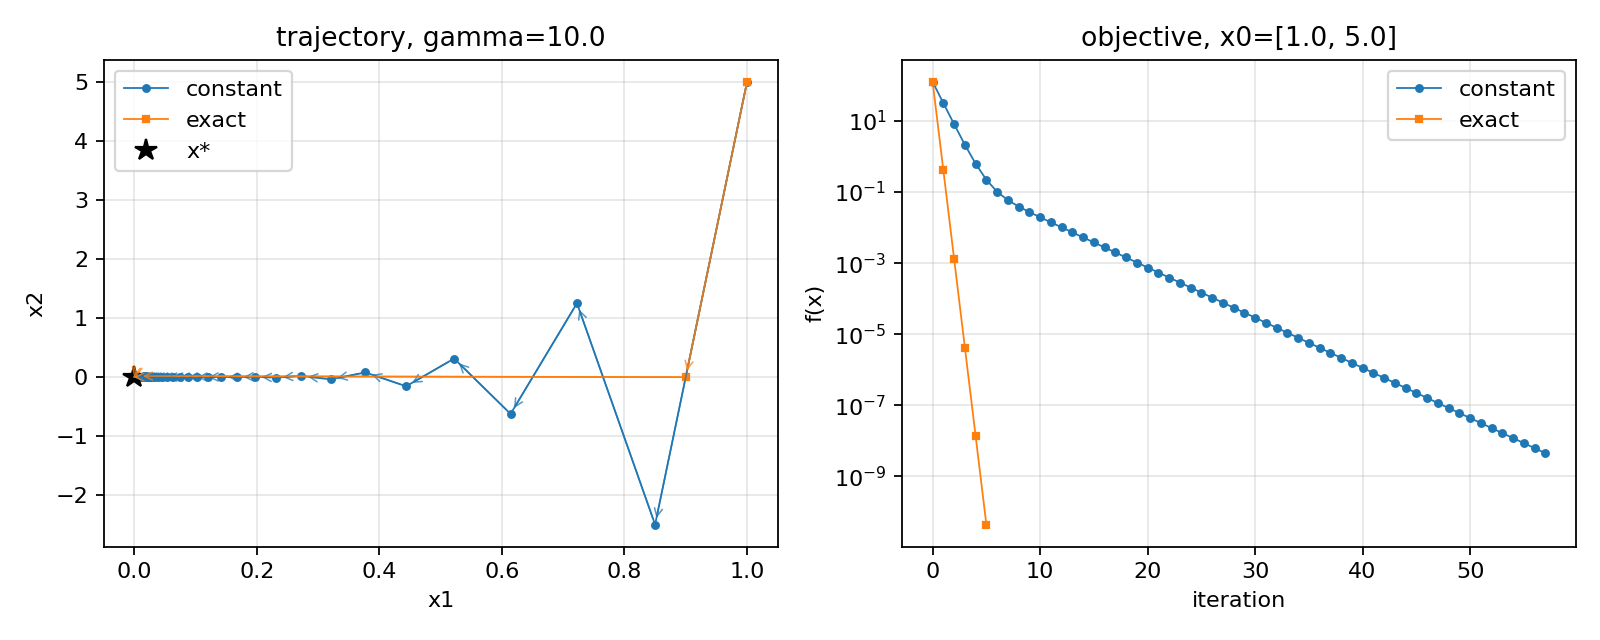
\includegraphics[width=0.82\textwidth]{code/p1_gamma10_x0_1_5.png}
    \caption{\(\gamma=10\), \(x^{(0)}=(1,5)\).}
\end{figure}

\begin{figure}[H]
    \centering
    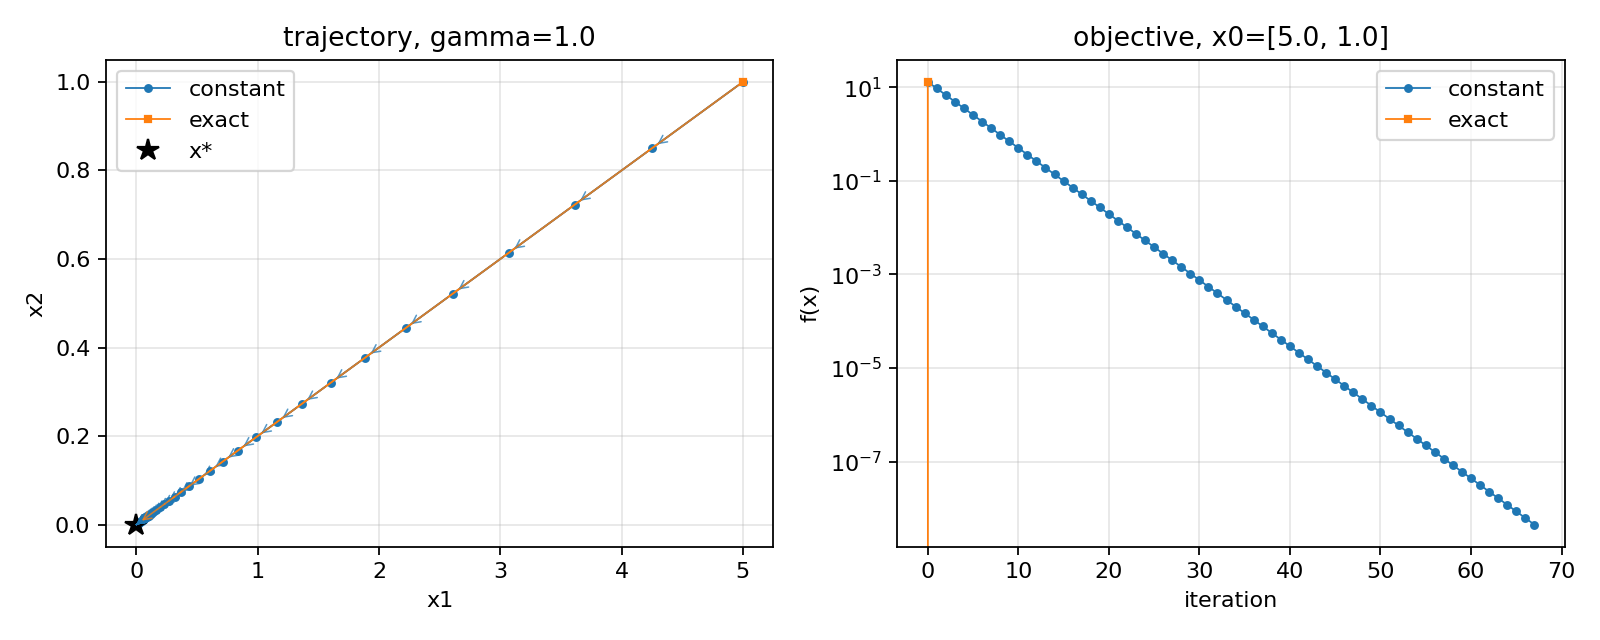
\includegraphics[width=0.82\textwidth]{code/p1_gamma1_x0_5_1.png}
    \caption{\(\gamma=1\), \(x^{(0)}=(5,1)\).}
\end{figure}

\begin{figure}[H]
    \centering
    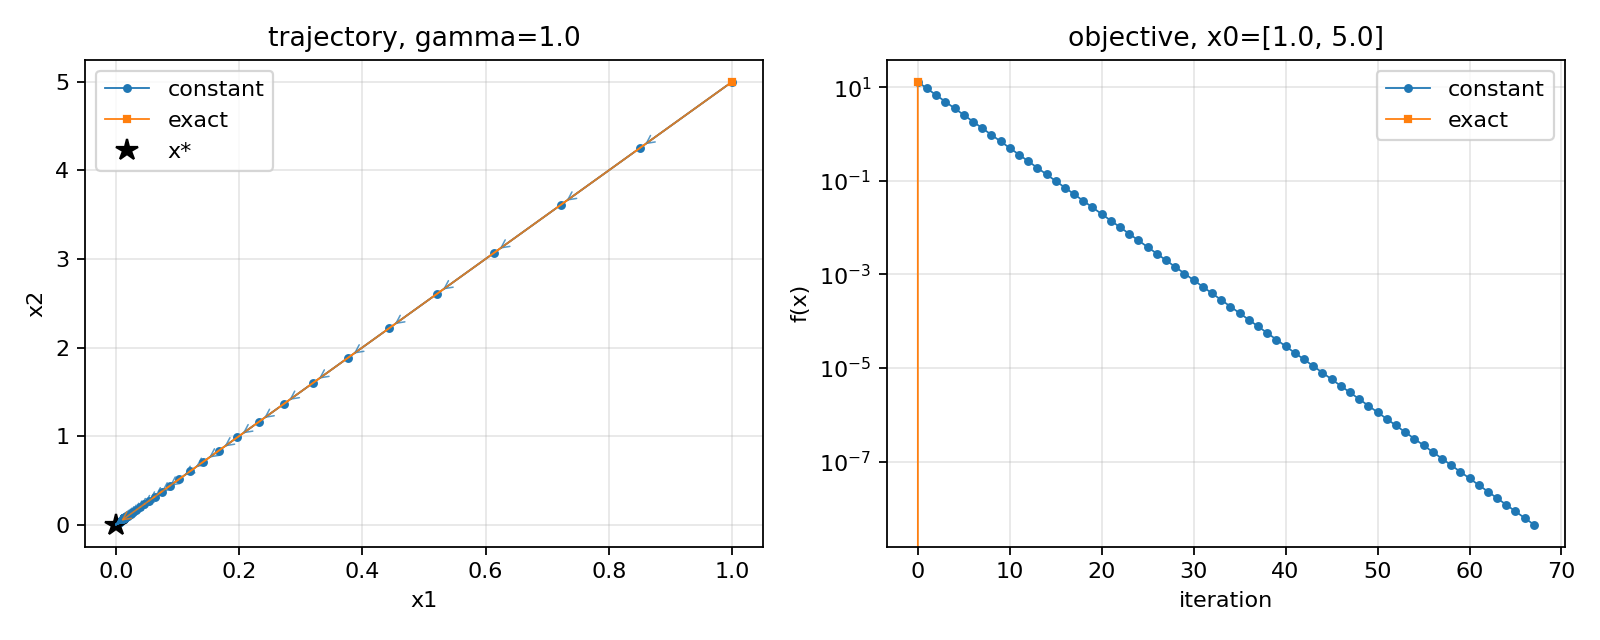
\includegraphics[width=0.82\textwidth]{code/p1_gamma1_x0_1_5.png}
    \caption{\(\gamma=1\), \(x^{(0)}=(1,5)\).}
\end{figure}

\textbf{Code:}

\begin{lstlisting}
def f(x, q, b):
    return 0.5 * x.T @ q @ x - b.T @ x

def grad_f(x, q, b):
    return q @ x - b

def gd_constant(x0, q, b, eta):
    x = x0.astype(float).copy()
    traj = [x.copy()]
    vals = [f(x, q, b)]
    tol = 1e-4

    while np.linalg.norm(grad_f(x, q, b)) > tol:
        g = grad_f(x, q, b)
        x = x - eta * g
        traj.append(x.copy())
        vals.append(f(x, q, b))

    return np.array(traj), np.array(vals)

def gd_exact_line_search(x0, q, b):
    x = x0.astype(float).copy()
    traj = [x.copy()]
    vals = [f(x, q, b)]
    tol = 1e-4

    while np.linalg.norm(grad_f(x, q, b)) > tol:
        d = -grad_f(x, q, b)
        eta = (d.T @ d) / (d.T @ q @ d)
        x = x + eta * d
        traj.append(x.copy())
        vals.append(f(x, q, b))

    return np.array(traj), np.array(vals)

def run(gamma, x0):
    q = np.diag([1.0, gamma])
    b = np.zeros(2)
    eta_const = 0.15
    traj_const, vals_const = gd_constant(x0, q, b, eta_const)
    traj_ls, vals_ls = gd_exact_line_search(x0, q, b)
\end{lstlisting}

\newpage

\subsection*{1.2(b)}

Using constant-step gradient descent with step size \(\eta=10^{-5}\).

The terminal output from the implementation is:

\begin{verbatim}
eta_const = 1.000000e-05
iterations = 279802
final objective = -27.052877
LQR cost J(u*) = 2.947123
\end{verbatim}


\textbf{Code:}

\begin{lstlisting}
T = 20
A = np.array([[1.0, 1.0], [0.0, 1.0]])
B = np.array([[0.0], [1.0]])
Q = np.eye(2)
R = np.eye(1)
Q_T = 10.0 * np.eye(2)
x0 = np.array([1.0, 0.0])

n = A.shape[0]
m = B.shape[1]
u0 = np.zeros(m * T)

nu = np.zeros((n * T, n))
V = np.zeros((n * T, m * T))

a_powers = [np.eye(n)]
for _ in range(T):
    a_powers.append(a_powers[-1] @ A)

for t in range(T):
    nu[t*n:(t+1)*n, :] = a_powers[t + 1]
    for k in range(t + 1):
        V[t*n:(t+1)*n, k*m:(k+1)*m] = a_powers[t - k] @ B

H = np.zeros((n * T, n * T))
for t in range(T - 1):
    H[t*n:(t+1)*n, t*n:(t+1)*n] = Q
H[(T - 1)*n:T*n, (T - 1)*n:T*n] = Q_T

N = np.zeros((m * T, m * T))
for t in range(T):
    N[t*m:(t+1)*m, t*m:(t+1)*m] = R

Q_tilde = 2.0 * (V.T @ H @ V + N)
b_tilde = -2.0 * V.T @ H @ nu @ x0

eta_const = 1e-5
traj_const, vals_const = gd_constant(u0, Q_tilde, b_tilde, eta_const)

u_star = traj_const[-1]
x_stack = nu @ x0 + V @ u_star
J_lqr = x0.T @ Q @ x0
for t in range(T - 1):
    x_t = x_stack[t*n:(t+1)*n]
    u_t = u_star[t*m:(t+1)*m]
    J_lqr += x_t.T @ Q @ x_t + u_t.T @ R @ u_t
x_T = x_stack[(T - 1)*n:T*n]
J_lqr += x_T.T @ Q_T @ x_T
\end{lstlisting}

\end{document}
